% ══════════════════════════════════════════════════════════════════════════════
% CHAPTER 3 — INSTITUTIONAL BACKGROUND
% ══════════════════════════════════════════════════════════════════════════════

This chapter describes the institutional features of the FOMC and
the ECB that are directly relevant to the measurement and
interpretation of monetary policy communication. Rather than
providing a general overview of each institution, the discussion
focuses on the structural characteristics that shape the textual
properties of the documents analysed in this thesis, generate
predictions about where FOMC and ECB results should differ, and
explain specific features of the data. (Do we need an introduction like this? I dont think its necessary maybe pelase remove)


% ══════════════════════════════════════════════════════════════════════════════
\section{The Federal Open Market Committee}
\label{sec:inst_fomc}
% ══════════════════════════════════════════════════════════════════════════════

\subsection{Mandate and Decision-Making}
\label{sec:inst_fomc_mandate}

The Federal Reserve operates under a \emph{dual mandate}: maximum
employment and price stability, as specified in Section~2A of the
Federal Reserve Act. This mandate has direct implications for FOMC
communication. Unlike the ECB, whose communication is more strongly
centred on price stability and inflation dynamics, FOMC statements and
press conferences regularly discuss labour-market conditions, wages,
unemployment, and hiring. The dictionary used in this thesis is therefore
constructed to capture employment-related language as one component of
hawkish--dovish tone, alongside policy-action, inflation, and residual
monetary-policy language. This does not imply separate FOMC and ECB
dictionaries; rather, the same cross-bank dictionary includes terms that
are relevant for both institutions, including terms that appear more
frequently in FOMC communication because of the Federal Reserve's dual
mandate.

The FOMC's decision-making structure also matters for the form of its
communication. The post-meeting statement is a committee product and is
therefore likely to be carefully negotiated and relatively formulaic. By
contrast, press conferences allow the Chair to explain the decision and
respond to questions in less scripted language. This distinction is
important for the empirical analysis because it suggests that statements
may exhibit a narrower distribution of tone scores, while press
conferences may contain more variation in hawkish--dovish language. The
score distributions in \Cref{sec:res_scores} provide a direct
check of this implication.

The FOMC normally holds eight scheduled meetings per year. The sample
also includes several unscheduled inter-meeting policy actions during
periods of acute financial stress, including 2001, 2008, and 2020. These
events are identified in the USMPD through the \texttt{Unscheduled}
indicator and are reported in the data description. They are not modeled
separately in the baseline regressions, but they are important for
interpreting the sample because they correspond to unusually large and
crisis-driven policy moves.

\subsection{Evolution of Communication Practices}
\label{sec:inst_fomc_evolution}

The evolution of FOMC communication is an important feature of the
sample, because the same text-scoring methods are applied across more
than three decades of changing communication practices. The sample begins
in February~1994, when the FOMC first issued a post-meeting statement.
The initial statement was short and mainly announced the policy action,
but statements gradually became longer and more explanatory over time.

A key development was the increasing use of forward-looking language.
From the late 1990s onward, FOMC statements began to include more
explicit assessments of risks and the likely future direction of policy.
During the 2004--2006 tightening cycle, phrases such as ``measured
pace'' provided guidance about the expected path of interest rates. After
the Global Financial Crisis, forward guidance became more explicit
through calendar-based and threshold-based language, such as commitments
to keep rates low for an extended period. Since 2007, the Summary of
Economic Projections has further increased the transparency of the
Committee's outlook, and since 2012 the dot plot has provided an
additional signal about participants' expected path of the federal funds
rate.

Press conferences add another layer of communication. They were
introduced in April~2011 under Chairman Bernanke and have been held
after every scheduled FOMC meeting since 2019. As a result, the FOMC
press-conference sample is shorter than the statement sample, covering
2011--2026 rather than 1994--2026. More recently, FOMC communication has
emphasised phrases such as ``data dependent'' and ``meeting by meeting'',
which signal conditionality rather than a fixed policy path.

This evolution poses a challenge for any fixed dictionary, because the
vocabulary of monetary policy changes over time. The forward/backward
sentence split used in this thesis is designed to capture broad
forward-looking language, including projections, commitments,
conditionality, and references to the future policy path. The Random
Forest and RoBERTa extensions provide additional benchmarks because they
are less dependent on a fixed hand-coded vocabulary than the dictionary
approach.


\subsection{Statements and Press Conferences as Analytical Objects}
\label{sec:inst_fomc_objects}

The two FOMC document types analysed in this thesis differ in their
textual properties and in the market windows to which they are matched.

\textbf{Statements} are short, highly structured, and carefully
negotiated committee documents. Their wording is therefore relatively
formulaic, and changes from one meeting to the next are closely watched
by market participants. This makes statements well suited for
dictionary-based measurement, because small changes in policy language
can be economically meaningful. At the same time, their brevity means
that each document contains fewer matched phrases and fewer informative
bigrams, which can make both dictionary scores and machine-learning
features more sensitive to small wording changes.

\textbf{Press conferences} are longer and less scripted. They include
prepared remarks by the Chair followed by responses to journalists'
questions. After cleaning, this thesis retains only the Chair's answers
and removes journalist questions, so that the measured tone reflects
central bank communication rather than the wording of the questions.
Because press conferences contain substantially more text and more varied
language than statements, they provide richer material for measuring
hawkish--dovish tone. They may also reveal how the Chair interprets
incoming data, risks, and policy trade-offs beyond the wording of the
statement.

The USMPD provides separate high-frequency event windows for FOMC
statements and press conferences. This allows the empirical analysis to
match each document type to the corresponding market reaction: statement
texts are matched to the statement window, while press-conference texts
are matched to the press-conference window. The dependent variables are
therefore high-frequency market reactions around the relevant
communication window, not daily price changes.


% ══════════════════════════════════════════════════════════════════════════════
\section{The European Central Bank}
\label{sec:inst_ecb}
% ══════════════════════════════════════════════════════════════════════════════

\subsection{Mandate and Decision-Making}
\label{sec:inst_ecb_mandate}

The ECB's primary objective is the maintenance of price stability. Until
the 2021 strategy review, price stability was defined as inflation below,
but close to, 2\% over the medium term. The revised strategy introduced
a symmetric 2\% inflation target. Compared with the Federal Reserve's
dual mandate, this institutional framework implies that ECB
communication is more strongly centred on inflation dynamics and price
stability, although the ECB also discusses real activity, labour markets,
credit conditions, and financial risks.

This distinction is relevant for the dictionary design. The same
cross-bank dictionary is applied to both the FOMC and the ECB, but the
relative importance of its components may differ across institutions.
Employment-related language is expected to play a larger role in FOMC
communication, while inflation and price-stability language should be
more central in ECB communication. The four-category decomposition
therefore allows the analysis to examine whether different dimensions of
tone matter across the two central banks.

The ECB's communication frequency also differs over the sample. Until
January~2015, monetary policy meetings were held monthly; since then,
they have followed a six-weekly cycle similar to the FOMC. This affects
the structure of the ECB sample, especially in the pre-2015 period, where
ECB communication events occur more frequently.

A further institutional difference concerns the ECB's policy rates. The
ECB operates with several policy rates, including the main refinancing
operations (MRO) rate and the deposit facility rate (DFR). This thesis
uses changes in the MRO rate as the single ECB rate-decision benchmark
in order to maintain a consistent measure across the full sample. This is
a simplification, particularly for the post-2014 period, when the deposit
facility rate became increasingly important. On several dates, the MRO
and DFR moved differently. These cases are discussed as a limitation in
\Cref{ch:discussion}. For the Random Forest classification exercise, any
negative rate change is treated as a ``cut'' and any positive change as a
``hike'', while the continuous forecasting regressions preserve the
actual basis-point magnitude.


\subsection{Communication Channels}
\label{sec:inst_ecb_channels}

The ECB's communication architecture differs from the FOMC's in ways
that are directly relevant for the empirical design.

The ECB policy statement, referred to as the ``statement'' in this
thesis, is delivered by the President at the start of the press
conference on behalf of the Governing Council. It summarises the policy
decision, the inflation outlook, real-economy developments, and broader
financial and monetary conditions. Compared with the FOMC statement, it
is more closely integrated with the press conference, since it serves as
the opening statement before the Q\&A session.

The ECB press conference has been part of the communication framework
since the beginning of monetary union in 1999. This creates an important
difference relative to the FOMC: the ECB press-conference corpus covers
the full 1999--2026 sample, while the FOMC press-conference corpus begins
only in 2011. The Q\&A section is led by the President and may include
responses from other senior ECB officials. In the cleaned corpus, the
analysis retains central-bank speakers' responses and removes journalist
questions, so that the measured tone reflects ECB communication rather
than the wording of the questions (\Cref{sec:data_ecb_pc}).


\subsection{Presidents and Communication Styles}
\label{sec:inst_ecb_presidents}

The ECB sample spans four presidencies: Wim Duisenberg
(1998--2003), Jean-Claude Trichet (2003--2011), Mario Draghi
(2011--2019), and Christine Lagarde (2019--present). These leadership
periods are relevant because communication style and policy vocabulary
changed substantially over time.

Under Trichet, ECB communication became known for coded policy language.
The phrase ``strong vigilance'', for example, was widely interpreted by
market participants as a signal that a rate hike could follow at the next
meeting. This illustrates why phrase-level measurement is useful:
specific bigrams can carry policy information that would be missed by
single-word counts.

Draghi's presidency marked a period in which communication became a more
visible policy instrument. The ``whatever it takes'' speech, the
introduction of explicit forward guidance, and the move to negative
rates all illustrate the growing role of language in shaping market
expectations. Under Lagarde, ECB communication has increasingly stressed
conditionality through phrases such as ``data dependent'' and
``meeting by meeting''. These expressions are included among the
forward-looking markers used in this thesis because they indicate that
future policy decisions depend on incoming information rather than on a
pre-committed rate path.

The empirical analysis accounts for these leadership differences by
including president-period fixed effects in robustness specifications.
This allows the tone--market relationship to be assessed after absorbing
persistent differences in communication style across ECB presidencies.

% ══════════════════════════════════════════════════════════════════════════════
\section{Comparative Analysis of Communication Frameworks}
\label{sec:inst_comparison}
% ══════════════════════════════════════════════════════════════════════════════

\subsection{Structural Differences and Analytical Implications}
\label{sec:inst_comparison_structure}

\Cref{tab:inst_comparison} summarises the key structural
differences between FOMC and ECB communication that are relevant
to the empirical analysis;
\Cref{fig:decision_making} visualises the decision-making
asymmetry that drives several of these differences.

\begin{table}[htbp]
\centering
\caption{Structural comparison of FOMC and ECB communication}
\label{tab:inst_comparison}
\begin{threeparttable}
\begin{tabular}{lll}
\toprule
Dimension & FOMC & ECB \\
\midrule
Mandate
  & Dual (employment + prices)
  & Single (prices) \\
Statement authorship
  & Committee consensus
  & President reads \\
Press conferences available
  & Since April 2011
  & Since January 1999 \\
Meeting frequency
  & 8/year (stable)
  & 12/year $\to$ 8/year (2015) \\
Rate change granularity
  & Multiples of 25 bps
  & Includes 5, 10 bps \\
Q\&A speakers
  & Chair only
  & President + board members \\
\bottomrule
\end{tabular}
\begin{tablenotes}\footnotesize
  \item[] These differences directly affect the textual properties
    of the documents, the sample composition, and the expected
    performance of the scoring methods.
\end{tablenotes}
\end{threeparttable}
\end{table}

% --------------------------------------------------------------------------
% Decision-making structure figure
% --------------------------------------------------------------------------

\begin{figure}[htbp]
\centering
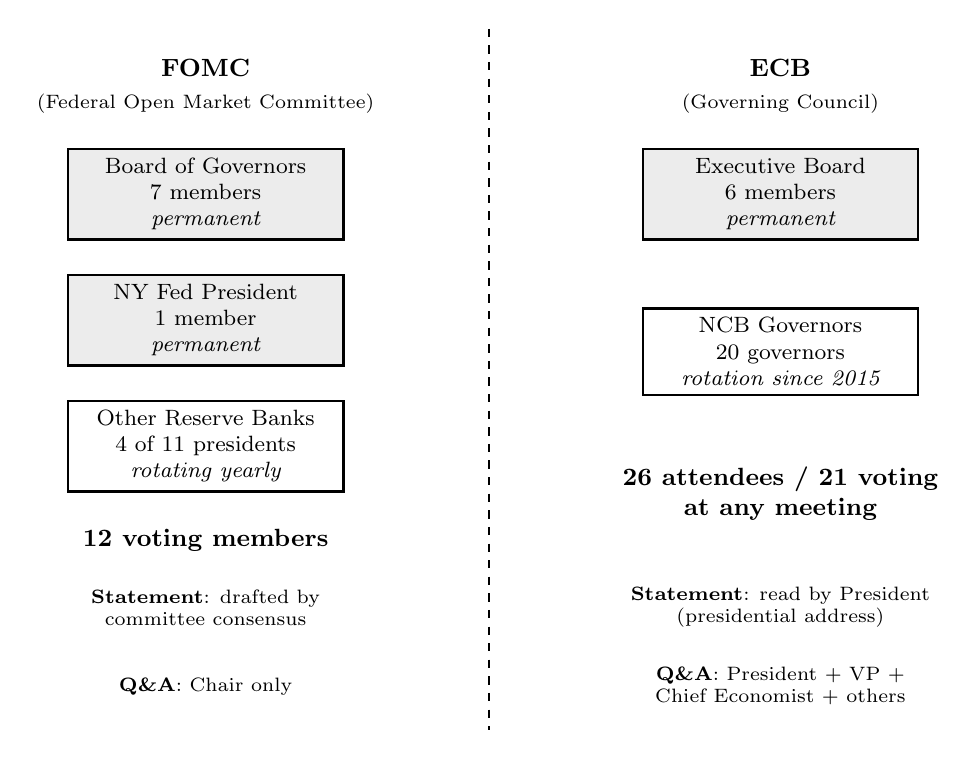
\begin{tikzpicture}[
    every node/.style={font=\footnotesize},
    boxstyle/.style={rectangle, draw=black, thick, minimum height=1.0cm,
                     minimum width=3.5cm, align=center, font=\footnotesize},
    permbox/.style={fill=gray!15},
    label/.style={font=\small\bfseries}
]
  % FOMC column
  \node[label] at (0, 5.0) {\textbf{FOMC}};
  \node[label, font=\scriptsize] at (0, 4.55) {(Federal Open Market Committee)};
  \node[boxstyle, permbox] (fomc-bog) at (0, 3.4) {Board of Governors\\7 members\\\itshape permanent};
  \node[boxstyle, permbox] (fomc-ny)  at (0, 1.8) {NY Fed President\\1 member\\\itshape permanent};
  \node[boxstyle]          (fomc-rot) at (0, 0.2) {Other Reserve Banks\\4 of 11 presidents\\\itshape rotating yearly};

  \node[font=\small\bfseries] at (0, -1.0) {12 voting members};
  \node[font=\scriptsize, align=center] at (0, -1.85)
    {\textbf{Statement}: drafted by\\committee consensus};
  \node[font=\scriptsize, align=center] at (0, -2.85)
    {\textbf{Q\&A}: Chair only};

  % Vertical separator
  \draw[thick, dashed] (3.6, 5.5) -- (3.6, -3.4);

  % ECB column
  \node[label] at (7.3, 5.0) {\textbf{ECB}};
  \node[label, font=\scriptsize] at (7.3, 4.55) {(Governing Council)};
  \node[boxstyle, permbox] (ecb-eb)  at (7.3, 3.4) {Executive Board\\6 members\\\itshape permanent};
  \node[boxstyle]          (ecb-ncb) at (7.3, 1.4) {NCB Governors\\20 governors\\\itshape rotation since 2015};

  \node[font=\small\bfseries, align=center] at (7.3, -0.4)
    {26 attendees / 21 voting\\at any meeting};
  \node[font=\scriptsize, align=center] at (7.3, -1.85)
    {\textbf{Statement}: read by President\\(presidential address)};
  \node[font=\scriptsize, align=center] at (7.3, -2.85)
    {\textbf{Q\&A}: President + VP +\\Chief Economist + others};

\end{tikzpicture}
\caption[Decision-making structures]{Decision-making structures of
the FOMC and the ECB Governing Council. Shaded boxes indicate
permanent voting members; unshaded boxes indicate rotating members. ( But again how does it really impact our thesis and our findings? Is that relevant for our thesis? That they are rotating or not)
The FOMC's smaller and predominantly permanent voting body
(12~members, of which 8 are permanent) produces a committee-drafted
statement in which every word is negotiated. The ECB's much larger
Council (26~attendees including 20 NCB governors since 2023, of
which 21 vote at any meeting under the rotation system introduced
in 2015) delegates statement preparation to the President. The Q\&A
composition mirrors this asymmetry: only the Chair speaks at FOMC
press conferences, while the ECB Q\&A typically includes responses
from the Vice-President and other Executive Board members.}
\label{fig:decision_making}
\end{figure}

% --------------------------------------------------------------------------
% Communication innovation milestones table
% --------------------------------------------------------------------------

\Cref{tab:comm_innovations} traces the parallel evolution of
FOMC and ECB communication practices over the sample period.
The two institutions have converged on broadly similar tools,
including explicit forward guidance, calendar- and state-contingent
commitments, post-meeting press conferences, and ``data dependent''
language during normalisation phases, but the timing of adoption
differs in ways that create asymmetric coverage in the sample.

\begin{threeparttable}
\begin{tablenotes}
  \item[] Selected milestones with direct relevance to the textual
    content analysed in this thesis. Phrases shown in quotation
    marks appear among the dictionary terms or forward-looking
    sentence markers
    (\Cref{sec:meth_dict_selection,sec:meth_fwd_bwd}).
\end{tablenotes}

\begin{longtable}{cp{6.0cm}p{6.0cm}}
\caption{Communication-innovation milestones, FOMC and ECB}
\label{tab:comm_innovations}\\
\toprule
Year & FOMC & ECB \\
\midrule
\endfirsthead

\multicolumn{3}{l}{\footnotesize\itshape Table~\ref{tab:comm_innovations} continued from previous page}\\
\toprule
Year & FOMC & ECB \\
\midrule
\endhead

\midrule
\multicolumn{3}{r}{\footnotesize\itshape continued on next page}\\
\endfoot

\bottomrule

\endlastfoot

1994 & First post-meeting statement (single sentence)
     & --- \\
\addlinespace
1999 & Balance-of-risks language introduced (1999--2000)
     & ECB founded; press conferences with Q\&A from
       inception; two-pillar strategy \\
\addlinespace
2003 & ---
     & First strategy review (HICP target reformulated as
       ``below, but close to, 2\%'') \\
\addlinespace
2004 & Forward-guidance phrases (``measured pace'') during
       gradual tightening cycle
     & --- \\
\addlinespace
2007 & ---
     & ``Strong vigilance'' established as virtual
       commitment to hike at next meeting \\
\addlinespace
2008 & Zero lower bound reached December 2008;
       calendar-based forward guidance (``for an extended
       period'')
     & First crisis-period rate cuts; coordinated October
       2008 cut \\
\addlinespace
2011 & First press conference (April; alternating meetings)
     & --- \\
\addlinespace
2012 & State-contingent forward guidance (``Evans rule'',
       Dec.\ 2012)
     & ``Whatever it takes'' (Draghi, July);
       Outright Monetary Transactions announced \\
\addlinespace
2013 & ---
     & First explicit forward guidance (``key ECB rates
       to remain at present or lower levels for an
       extended period of time'') \\
\addlinespace
2014 & ---
     & Deposit facility rate enters negative territory
       (June) \\
\addlinespace
2015 & ---
     & Asset Purchase Programme launched (January);
       voting rotation system activated; switch to
       six-weekly meetings \\
\addlinespace
2019 & Press conferences extended to every meeting (January)
     & --- \\
\addlinespace
2020 & FAIT framework adopted (August); emergency rate cuts
       to ZLB
     & Pandemic Emergency Purchase Programme (March) \\
\addlinespace
2021 & ---
     & Strategy review concluded; symmetric 2\% target
       adopted \\
\addlinespace
2022 & ``Data dependent'' / ``meeting by meeting'' language
       returns; fastest tightening cycle in 40 years
     & Tightening cycle begins (July); ``data dependent''
       and ``meeting by meeting'' language adopted \\
\end{longtable}
\end{threeparttable}

Several of these structural differences generate specific
predictions for the empirical results.

First, the \emph{dual mandate} of the FOMC implies that its
communications should contain a richer vocabulary related to
employment and output, whereas ECB communications should be more
narrowly focused on inflation and prices. The dictionary's
inclusion of employment-related terms may therefore produce more
hawkish and dovish matches in FOMC texts than in ECB texts,
potentially leading to wider score distributions for the FOMC.

Second, the \emph{committee-consensus nature} of FOMC statements
predicts lower lexical variance and a narrower distribution of
net scores compared with press conferences, where the Chair speaks
with less constraint. For the ECB, where the statement is
also a controlled product, a similar pattern is expected.

Third, the \emph{asymmetric press conference coverage} (ECB press
conferences from 1999 versus FOMC press conferences from 2011)
means that the ECB press conference results are based on a
substantially larger sample and cover more monetary policy regimes.

Fourth, the ECB's \emph{non-standard rate changes} ($-5$ and
$-10$~bps) create a more heterogeneous ``cut'' class for the
Random Forest classifier, which may make it harder to learn
cut-specific language patterns compared with the FOMC's uniform
25-bp increments.


\subsection{Implications for Scoring Methodology}
\label{sec:inst_comparison_scoring}

These institutional differences have direct implications for the three
scoring approaches used in this thesis.

For the \emph{dictionary}, the key question is whether one common
vocabulary can capture hawkish--dovish tone across two institutions with
different mandates and communication styles. The dictionary was
constructed by combining monetary-policy terms identified from FOMC and
ECB communication with hand-curated phrase selection. In practice, this
means that frequently used policy-relevant expressions were inspected and
assigned to hawkish or dovish categories where they carried a clear
stance signal. Because the same dictionary is applied to all corpora,
mandate-specific language may be captured differently across the FOMC
and ECB samples. The agreement analysis in \Cref{sec:res_agreement_new} 
therefore examines how well the dictionary classifications align with
policy decisions across the four corpora.

For the \emph{Random Forest}, separate models are estimated for each
corpus. This allows the classifier to learn institution-specific and
document-type-specific bigram patterns. The Random Forest can therefore
adapt to differences between FOMC statements, FOMC press conferences,
ECB statements, and ECB press conferences, whereas the dictionary applies
the same fixed vocabulary to all documents.

For the \emph{RoBERTa-based classifier}, the thesis uses sentence-level
hawkish, dovish, and neutral predictions to construct document-level tone
scores. This provides a contextual benchmark against the dictionary and
Random Forest approaches, since the classification is based on sentence
meaning rather than fixed phrase counts. Because the prediction files are
applied to both FOMC and ECB texts, the comparison also indicates whether
the contextual classifier produces useful tone measures across different
central bank communication styles.

The three-way comparison in \Cref{sec:res_rq1_new} tests whether the
Random Forest's corpus-specific feature learning and RoBERTa's
sentence-level contextual classification provide additional explanatory
power relative to the transparent but static dictionary approach.


% ══════════════════════════════════════════════════════════════════════════════
\section{Monetary Policy Regimes}
\label{sec:inst_eras}
% ══════════════════════════════════════════════════════════════════════════════

To contextualise the results across different macroeconomic and monetary
policy environments, the thesis defines broad policy eras for each
central bank. \Cref{fig:era_timeline} shows the FOMC and ECB era
boundaries on a common timeline, while \Cref{tab:era_dates} reports the
corresponding cutoff dates. \Cref{fig:rate_paths} plots the policy-rate
paths and illustrates how the era definitions relate to major shifts in
the monetary policy environment.

These era classifications are used in three parts of the analysis. The
data chapter reports the distribution of rate decisions by era
(\Cref{tab:rate_by_era}). The methodology chapter introduces era fixed
effects as a robustness specification for the market-reaction
regressions (\Cref{sec:meth_rq1}). The results chapter uses the same
classification to examine whether tone measures behave differently
across monetary policy environments.

\begin{figure}[htbp]
\centering
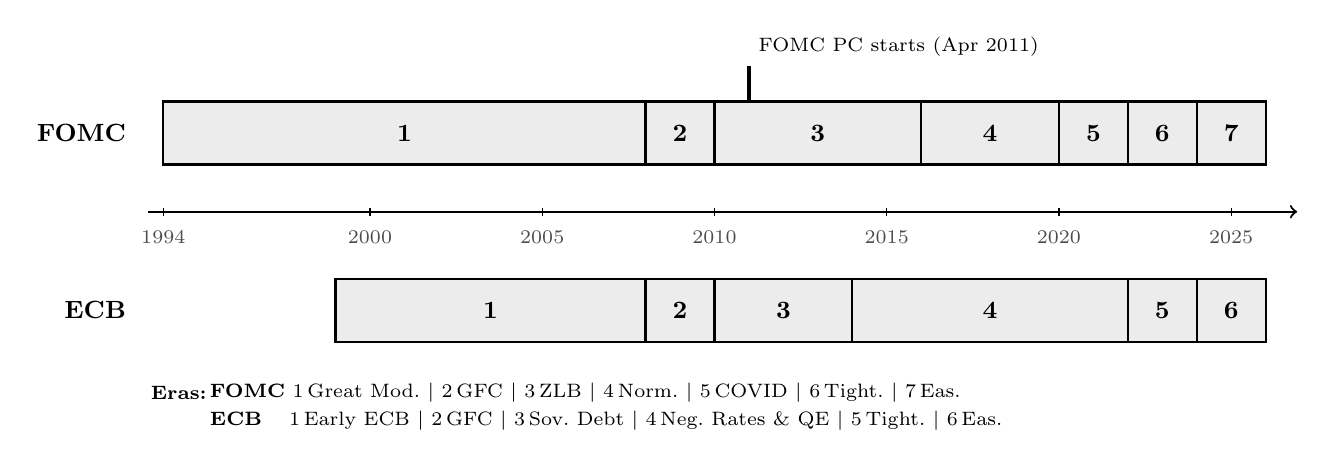
\begin{tikzpicture}[
    every node/.style={font=\footnotesize},
    yearmark/.style={font=\scriptsize, black!70},
    eranum/.style={font=\small\bfseries, black, anchor=center},
    fomcera/.style={fill=gray!15, draw=black, thick},
    ecbera/.style={fill=gray!15, draw=black, thick},
    banklabel/.style={anchor=east, font=\small\bfseries, black},
    pcmarker/.style={font=\scriptsize, anchor=south west, black},
    keyitem/.style={font=\scriptsize, anchor=west, inner sep=1pt}
]
\def\xstart{0}
\def\xend{14}
\pgfmathsetmacro{\unit}{(\xend-\xstart)/(2026-1994)}

\draw[->, thick] (\xstart-0.2, 0) -- (\xend+0.4, 0);
\foreach \y in {1994, 2000, 2005, 2010, 2015, 2020, 2025} {
  \pgfmathsetmacro{\xpos}{\xstart + (\y-1994)*\unit}
  \draw (\xpos, -0.05) -- (\xpos, 0.05);
  \node[yearmark, below=2pt] at (\xpos, -0.05) {\y};
}

\foreach \start/\end/\num in {%
  1994/2008/1, 2008/2010/2, 2010/2016/3, 2016/2020/4,%
  2020/2022/5, 2022/2024/6, 2024/2026/7}{
  \pgfmathsetmacro{\xa}{\xstart + (\start-1994)*\unit}
  \pgfmathsetmacro{\xb}{\xstart + (\end-1994)*\unit}
  \draw[fomcera] (\xa, 0.6) rectangle (\xb, 1.4);
  \node[eranum] at ({(\xa+\xb)/2}, 1.0) {\num};
}
\node[banklabel] at (\xstart-0.35, 1.0) {FOMC};

\foreach \start/\end/\num in {%
  1999/2008/1, 2008/2010/2, 2010/2014/3, 2014/2022/4,%
  2022/2024/5, 2024/2026/6}{
  \pgfmathsetmacro{\xa}{\xstart + (\start-1994)*\unit}
  \pgfmathsetmacro{\xb}{\xstart + (\end-1994)*\unit}
  \draw[ecbera] (\xa, -0.85) rectangle (\xb, -1.65);
  \node[eranum] at ({(\xa+\xb)/2}, -1.25) {\num};
}
\node[banklabel] at (\xstart-0.35, -1.25) {ECB};

\pgfmathsetmacro{\xfomcpc}{\xstart + (2011-1994)*\unit}
\draw[black, very thick] (\xfomcpc, 1.4) -- (\xfomcpc, 1.85);
\node[pcmarker] at (\xfomcpc, 1.85) {FOMC PC starts (Apr 2011)};

\node[keyitem, font=\scriptsize\bfseries] at (\xstart-0.2, -2.30) {Eras:};
\node[keyitem] at (\xstart+0.55, -2.30)
  {\textbf{FOMC} 1\,Great Mod.\ \textbar{} 2\,GFC \textbar{} 3\,ZLB \textbar{} 4\,Norm.\ \textbar{} 5\,COVID \textbar{} 6\,Tight.\ \textbar{} 7\,Eas.};
\node[keyitem] at (\xstart+0.55, -2.65)
  {\textbf{ECB}\;\;\,\, 1\,Early ECB \textbar{} 2\,GFC \textbar{} 3\,Sov.\ Debt \textbar{} 4\,Neg.\ Rates \& QE \textbar{} 5\,Tight.\ \textbar{} 6\,Eas.};

\end{tikzpicture}
\caption{FOMC and ECB monetary policy eras, 1994--2026. Era
boundaries follow the cutoff dates in \Cref{tab:era_dates}; both
bands use the same time scale. The vertical mark above the FOMC
band shows the start of the FOMC press conference sample
(April~2011); FOMC statements are available from February~1994,
and both ECB statements and press conferences from January~1999,
so the corresponding starts coincide with the left edge of each
band. The numbered key below the timeline names each era. Era
abbreviations: ZLB~$=$~Zero Lower Bound; Norm.~$=$~Normalisation;
Tight.~$=$~Post-COVID Tightening; Eas.~$=$~Easing Cycle.}
\label{fig:era_timeline}
\end{figure}

% --------------------------------------------------------------------------
% Policy rate paths figure
% --------------------------------------------------------------------------

\begin{figure}[htbp]
\centering
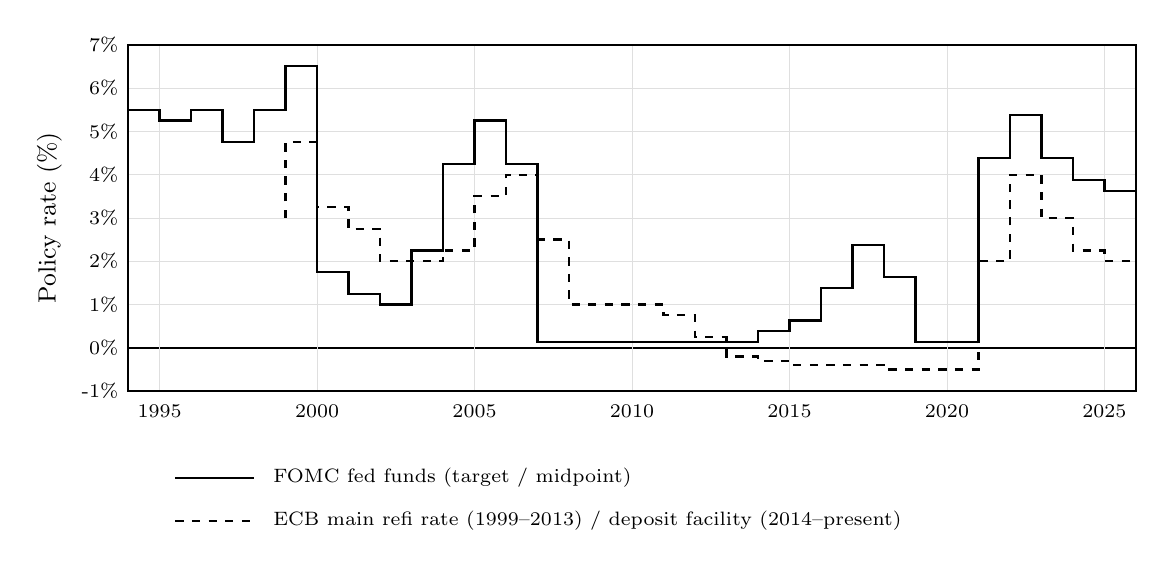
\begin{tikzpicture}[
    xscale=0.40, yscale=0.55,
    every node/.style={font=\scriptsize}
]
  \def\xmin{0}
  \def\xmax{32}
  \def\ymin{-1}
  \def\ymax{7}

  \foreach \y in {-1, 0, 1, 2, 3, 4, 5, 6, 7} {
    \draw[gray!25, very thin] (\xmin, \y) -- (\xmax, \y);
    \node[anchor=east] at (\xmin, \y) {\y\%};
  }
  \draw[black, thick] (\xmin, 0) -- (\xmax, 0);

  \foreach \xoff/\year in {%
    1/1995, 6/2000, 11/2005, 16/2010, 21/2015, 26/2020, 31/2025}{
    \draw[gray!25, very thin] (\xoff, \ymin) -- (\xoff, \ymax);
    \node[anchor=north] at (\xoff, \ymin-0.1) {\year};
  }

  \draw[thick] (\xmin, \ymin) rectangle (\xmax, \ymax);

  \draw[black, thick] plot[const plot mark right] coordinates {
    (0, 3.00)  (0.92, 5.50) (1, 5.50)  (2, 5.25)  (3, 5.50)
    (4, 4.75)  (5, 5.50)    (6, 6.50)  (7, 1.75)  (8, 1.25)
    (9, 1.00)  (10, 2.25)   (11, 4.25) (12, 5.25) (13, 4.25)
    (14, 0.13) (15, 0.13)   (16, 0.13) (17, 0.13) (18, 0.13)
    (19, 0.13) (20, 0.13)   (21, 0.38) (22, 0.63) (23, 1.38)
    (24, 2.38) (25, 1.63)   (26, 0.13) (27, 0.13) (28, 4.38)
    (29, 5.38) (30, 4.38)   (31, 3.88) (32, 3.63)
  };

  \draw[black, thick, dashed] plot[const plot mark right] coordinates {
    (5, 3.00)   (6, 4.75)   (7, 3.25)   (8, 2.75)   (9, 2.00)
    (10, 2.00)  (11, 2.25)  (12, 3.50)  (13, 4.00)  (14, 2.50)
    (15, 1.00)  (16, 1.00)  (17, 1.00)  (18, 0.75)  (19, 0.25)
    (20, -0.20) (21, -0.30) (22, -0.40) (23, -0.40) (24, -0.40)
    (25, -0.50) (26, -0.50) (27, -0.50) (28, 2.00)  (29, 4.00)
    (30, 3.00)  (31, 2.25)  (32, 2.00)
  };

  \draw[black, thick]         (1.5, \ymin-2.0) -- (4.0, \ymin-2.0);
  \node[anchor=west, font=\scriptsize] at (4.3, \ymin-2.0)
    {FOMC fed funds (target / midpoint)};
  \draw[black, thick, dashed] (1.5, \ymin-3.0) -- (4.0, \ymin-3.0);
  \node[anchor=west, font=\scriptsize] at (4.3, \ymin-3.0)
    {ECB main refi rate (1999--2013) / deposit facility (2014--present)};

  \node[rotate=90, font=\small] at (\xmin-2.5, 3) {Policy rate (\%)};
\end{tikzpicture}
\caption[Policy rate paths]{FOMC and ECB headline policy-rate
paths, 1994--2026. The solid line shows the FOMC's federal funds
target rate (target midpoint after the move to a target range in
December~2008). The dashed line shows the ECB's binding policy
rate: the main refinancing operations rate through May~2014, and
the deposit facility rate from June~2014 onward. The bold
horizontal line at zero marks the zero lower bound reference.}
\label{fig:rate_paths}
\end{figure}

\begin{table}[htbp]
\centering
\caption{Monetary policy era cutoff dates}
\label{tab:era_dates}
\begin{threeparttable}
\begin{tabular}{cll}
\toprule
\# & FOMC era (start--end) & ECB era (start--end) \\
\midrule
1 & Great Moderation, 1994-02 -- 2007-12     & Early ECB, 1999-01 -- 2007-12 \\
2 & GFC, 2008-01 -- 2009-12                  & GFC, 2008-01 -- 2009-12 \\
3 & Zero Lower Bound, 2010-01 -- 2015-12     & Sovereign Debt, 2010-01 -- 2013-12 \\
4 & Normalisation, 2016-01 -- 2019-12        & Negative Rates \& QE, 2014-01 -- 2021-12 \\
5 & COVID \& Recovery, 2020-01 -- 2021-12    & Post-COVID Tightening, 2022-01 -- 2023-12 \\
6 & Post-COVID Tightening, 2022-01 -- 2023-12 & Easing Cycle, 2024-01 -- present \\
7 & Easing Cycle, 2024-01 -- present         & --- \\
\bottomrule
\end{tabular}
\begin{tablenotes}\footnotesize
  \item[] End dates inclusive. Assignment is performed by the
    \texttt{add\_chair\_era()} helper in the data pipeline. The
    seven FOMC and six ECB eras listed here serve descriptive and
    narrative purposes. For the fixed-effects regressions in
    \Cref{sec:meth_fe}, these are collapsed into three broader
    periods: \emph{pre-GFC} (before 15~September~2008),
    \emph{ZLB and QE} (15~September~2008 to 31~December~2021),
    and \emph{post-ZLB} (from 1~January~2022). The coarser
    classification ensures sufficient observations per cell
    while capturing the structural breaks most relevant to the
    textual analysis.
\end{tablenotes}
\end{threeparttable}
\end{table}


\subsection{Era Descriptions}
\label{sec:inst_eras_descriptions}

The FOMC sample is divided into seven broad monetary policy eras. The
\emph{Great Moderation} period (1994--2007) covers the pre-crisis era of
relatively stable inflation and conventional interest-rate policy, with
shorter and more formulaic statements. The \emph{Global Financial Crisis}
period (2008--2009) captures the emergency easing cycle and the move
toward the zero lower bound. The \emph{Zero Lower Bound} era
(2010--2015) is characterised by constrained policy rates, large-scale
asset purchases, and an expanded role for forward guidance. The
\emph{Normalisation} period (2016--2019) covers the gradual tightening
cycle and increasing emphasis on data dependence. The \emph{COVID and
Recovery} era (2020--2021) includes emergency rate cuts, renewed asset
purchases, and communication around the recovery and inflation outlook.
The \emph{Post-COVID Tightening} period (2022--2023) captures the rapid
shift toward restrictive policy in response to elevated inflation.
Finally, the \emph{Post-Tightening/Easing} period (2024--2026) captures
the transition away from peak policy restrictiveness.

The ECB sample is divided into six broad eras. The \emph{Early ECB}
period (1999--2007) covers the institution's founding years and the
pre-crisis phase of conventional monetary policy. The \emph{Global
Financial Crisis} period (2008--2009) captures the ECB's response to the
financial crisis, including rate cuts and liquidity measures. The
\emph{Sovereign Debt Crisis} period (2010--2013) reflects the euro-area
debt crisis and the emergence of ECB-specific communication around
financial fragmentation and the integrity of the euro area. The
\emph{Negative Rates and QE} era (2014--2021) covers the period of
negative policy rates, asset purchases, and extended forward guidance.
The \emph{Post-COVID Tightening} period (2022--2023) captures the rapid
normalisation and tightening of policy in response to high inflation.
The final \emph{Post-Tightening/Easing} period (2024--2026) captures the
subsequent transition after the peak of the tightening cycle.


\subsection{The Role of Era Analysis}
\label{sec:inst_eras_role}

The era definitions serve two analytical purposes. First, they provide a
way to assess whether the tone measures behave differently across
monetary policy environments. In the results chapter, agreement between
tone classifications and rate decisions is reported by era where
relevant. This helps identify whether the dictionary, Random Forest, and
RoBERTa measures perform similarly across conventional policy periods,
zero-lower-bound episodes, crisis periods, and tightening cycles.

Second, the era structure helps interpret the time-series plots of the
dictionary, Random Forest, and BERT scores
(\Cref{sec:res_scores} and~\Cref{sec:res_rf_new}). Rather than
treating the full sample as homogeneous, the era definitions allow score
movements to be read against major shifts in the policy environment. This
makes it possible to assess whether the measures capture broad
transitions between dovish, neutral, and hawkish communication over time.